\section{Entity}

\begin{figure}[h]
\centering
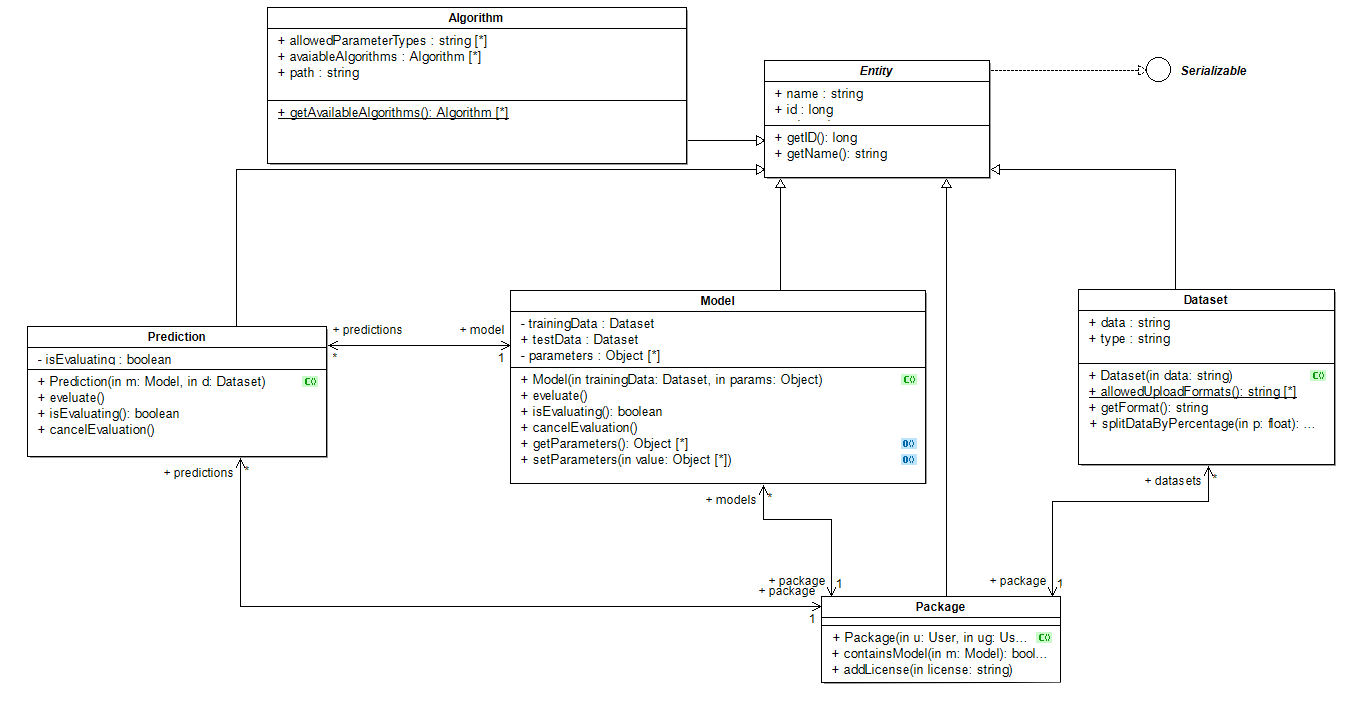
\includegraphics[width=1.0\linewidth]{Grafik/Klassendiagramme/Entity.png}
\caption{Abstrakte Superklasse}
\end{figure}

Jedes Package, Dataset, Model, jeder Algorithm und jede Prediction leiten von der Klasse Entity ab und haben somit einen eindeutige id, sowie uri und einen Namen. Über die Kommunikation mit den darüber liegenden Schichten wird der PluginLoader instruiert je nach Bedarf die jeweilig angeforderten Entities zu erzeugen bzw. abzurufen. Durch die Anbindung an die Weka-Library können die Datsets oder die Models verarbeitet werden, um so neue Predictions zu generieren.
Sämtliche administrativen Anfragen die den User oder Usergoups betreffen werden durch den UserManager gehandhabt. Dieser kooperiert über den Adapter mit dem PrivilegeManager, dem PackageManager und dem SecurityManager um die Anfragen zu beantworten.
Der Datenzugriff auf die Datenbank erfolgt vollständig über die Klasse Dataaccess, die ebenfalls an den Adapter angebunden ist. Diese Klasse bildet hierbei einen Wrapper um die SPARQL Abfragesprache um die Anfragen an die Datenbank zu formulieren und gewährleistet somit, dass keine gleichzeitigen Zugriffe auf die Datenbank erfolgen können, die zu Beschädigung führen könnten.